%% abtex2-modelo-trabalho-academico.tex, v<VERSION> laurocesar
%% Copyright 2012-<COPYRIGHT_YEAR> by abnTeX2 group at http://www.abntex.net.br/ 
%% This work may be distributed and/or modified under the conditions of the LaTeX Project Public License, either version 1.3 of this license or (at your option) any later version.
%% The latest version of this license is in http://www.latex-project.org/lppl.txt and version 1.3 or later is part of all distributions of LaTeX version 2005/12/01 or later.
%% The Current Maintainer of this work is the abnTeX2 team, led by Lauro César Araujo. Further information are available on http://www.abntex.net.br/

\documentclass[
	% -- opções da classe memoir --
	12pt,	% tamanho da fonte
	%openany,
	openright,			% capítulos começam em pág ímpar (insere página vazia caso preciso)
	%twoside,			% para impressão em recto e verso. Oposto a oneside
	oneside,            % para impressão em apenas um lado. Oposto twoside
	a4paper,			% tamanho do papel. 
	% -- opções da classe abntex2 --
	%chapter=TITLE,		% títulos de capítulos convertidos em letras maiúsculas
	%section=TITLE,		% títulos de seções convertidos em letras maiúsculas
	%subsection=TITLE,	% títulos de subseções convertidos em letras maiúsculas
	%subsubsection=TITLE,% títulos de subsubseções convertidos em letras maiúsculas
	% -- opções do pacote babel --
	english,			% idioma adicional para hifenização
	french,				% idioma adicional para hifenização
	spanish,			% idioma adicional para hifenização
	brazil				% o último idioma é o principal do documento
]{abntex2}

% ---
% Pacotes básicos 
% ---
\usepackage{lmodern}			% Usa a fonte Latin Modern			
\usepackage[T1]{fontenc}		% Selecao de codigos de fonte.
\usepackage[utf8]{inputenc}		% Codificacao do documento (conversão automática dos acentos)
\usepackage{indentfirst}		% Indenta o primeiro parágrafo de cada seção.
\usepackage{color}				% Controle das cores
\usepackage{graphicx}			% Inclusão de gráficos
\usepackage{microtype} 			% para melhorias de justificação
\usepackage{tablefootnote}      %inserir notas de rodapé em tabelas

%para usar codeblock
\usepackage{listings}
\definecolor{dkgreen}{rgb}{0,0.6,0}
\definecolor{gray}{rgb}{0.5,0.5,0.5}
\definecolor{mauve}{rgb}{0.58,0,0.82}
\lstset{frame=tb,
  language=Python,
  aboveskip=3mm,
  belowskip=3mm,
  showstringspaces=false,
  columns=flexible,
  basicstyle={\small\ttfamily},
  numbers=left,
  numberstyle=\tiny\color{gray},
  keywordstyle=\color{blue},
  commentstyle=\color{dkgreen},
  stringstyle=\color{mauve},
  breaklines=true,
  breakatwhitespace=true,
  tabsize=3
} 

% ---
		
% ---
% Pacotes adicionais, usados apenas no âmbito do Modelo Canônico do abnteX2
% ---
\usepackage{lipsum}	% para geração de dummy text
% ---

% ---
% Capa e folha de rosto personalizada
% ---
\usepackage{unijui}
% ---


% ---
% Pacotes de citações
% ---
\usepackage[brazilian,hyperpageref]{backref}	 % Paginas com as citações na bibl
\usepackage[alf]{abntex2cite}	% Citações padrão ABNT

% --- 
% CONFIGURAÇÕES DE PACOTES
% --- 

% ---
% Configurações do pacote backref
% Usado sem a opção hyperpageref de backref
\renewcommand{\backrefpagesname}{Citado na(s) página(s):~}
% Texto padrão antes do número das páginas
\renewcommand{\backref}{}
% Define os textos da citação
\renewcommand*{\backrefalt}[4]{
	\ifcase #1 %
		Nenhuma citação no texto.%
	\or
		Citado na página #2.%
	\else
		Citado #1 vezes nas páginas #2.%
	\fi}%
% ---

% ---
% Informações de dados para CAPA e FOLHA DE ROSTO
% ---
\titulo{Sistema de sugestão de produtos para e-commerce utilizando Inteligência Artificial}
\autor{Gabriel Cavalheiro Ullmann}
\local{Santa Rosa - RS}
\data{2020}
\orientador{Prof. Dr. Edson Luiz Padoin}
\instituicao{
  UNIVERSIDADE REGIONAL DO NOROESTE DO \\ESTADO DO RIO GRANDE DO SUL

    DEPARTAMENTO DE CIÊNCIAS EXATAS E ENGENHARIAS \\
    CIÊNCIA DA COMPUTAÇÃO}
\tipotrabalho{Monografia}
% O preambulo deve conter o tipo do trabalho, o objetivo, 
% o nome da instituição e a área de concentração 
\preambulo{Trabalho de Conclusão de Curso do curso de graduação em
Ciência da Computação apresentado ao Departamento de Ciências Exatas e Engenharias da Universidade Regional do Noroeste do Estado do Rio Grande do Sul como requisito parcial para a obtenção do título de Bacharel em Ciência da Computação.}
% ---


% ---
% Configurações de aparência do PDF final

% alterando o aspecto da cor azul
\definecolor{blue}{RGB}{41,5,195}

% informações do PDF
\makeatletter
\hypersetup{
     	%pagebackref=true,
		pdftitle={\@title}, 
		pdfauthor={\@author},
    	pdfsubject={\imprimirpreambulo},
	    pdfcreator={LaTeX with abnTeX2},
		pdfkeywords={abnt}{latex}{abntex}{abntex2}{trabalho acadêmico}, 
		colorlinks=false,       		% false: boxed links; true: colored links
    	linkcolor=blue,          	% color of internal links
    	citecolor=blue,        		% color of links to bibliography
    	filecolor=magenta,      		% color of file links
		%urlcolor=blue,
		urlcolor=black
		bookmarksdepth=4
}
\makeatother
% --- 

% ---
% Posiciona figuras e tabelas no topo da página quando adicionadas sozinhas
% em um página em branco. Ver https://github.com/abntex/abntex2/issues/170
\makeatletter
\setlength{\@fptop}{5pt} % Set distance from top of page to first float
\makeatother
% ---

% ---
% Possibilita criação de Quadros e Lista de quadros.
% Ver https://github.com/abntex/abntex2/issues/176
%
\newcommand{\quadroname}{Quadro}
\newcommand{\listofquadrosname}{Lista de quadros}

\newfloat[chapter]{quadro}{loq}{\quadroname}
\newlistof{listofquadros}{loq}{\listofquadrosname}
\newlistentry{quadro}{loq}{0}

% configurações para atender às regras da ABNT
\setfloatadjustment{quadro}{\centering}
\counterwithout{quadro}{chapter}
\renewcommand{\cftquadroname}{\quadroname\space} 
\renewcommand*{\cftquadroaftersnum}{\hfill--\hfill}

% ---
% Comandos personalizados: citar com tradução (com/sem parênteses)
% ---
\newcommand{\citedirt}[1]{\citeauthor{#1} (\citeyear{#1}, tradução nossa)}
\newcommand{\citedirtp}[1]{(\citeauthor{#1}, \citeyear{#1}, tradução nossa)}
% ---
% Comandos personalizados: citar sem tradução (com/sem parênteses)
% ---
\newcommand{\citedir}[1]{\citeauthor{#1} (\citeyear{#1})}
\newcommand{\citedir}[1]{(\citeauthor{#1} \citeyear{#1})}

% ---
% Ver https://github.com/abntex/abntex2/issues/176
% ---
\setfloatlocations{quadro}{hbtp} 

% --- 
% Espaçamentos entre linhas e parágrafos 
% --- 
\setlength{\parindent}{1.3cm}
\setlength{\parskip}{0.2cm} 

% ---
% compila o indice
% ---
\makeindex

% ----
% Início do documento
% ----
\begin{document}

% Seleciona o idioma do documento (conforme pacotes do babel)
\selectlanguage{brazil}

% Retira espaço extra obsoleto entre as frases.
\frenchspacing 

% ----------------------------------------------------------
% ELEMENTOS PRÉ-TEXTUAIS
% ----------------------------------------------------------
% \pretextual

% ---
% Capa
% ---

\imprimircapa
% ---

% ---
% Folha de rosto
% O símbolo * indica que haverá a ficha bibliográfica
% ---
\imprimirfolhaderosto*
% ---

% ---
% Inserir a ficha bibliografica
% ---
\begin{fichacatalografica}
	\sffamily
	\vspace*{\fill}					% Posição vertical
	\begin{center}					% Minipage Centralizado
	\fbox{\begin{minipage}[c][8cm]{13.5cm}		% Largura
	\small
	\imprimirautor
	%Sobrenome, Nome do autor
	
	\hspace{0.5cm} \imprimirtitulo  / \imprimirautor. --
	\imprimirlocal, \imprimirdata-
	
	\hspace{0.5cm} \thelastpage p. : il. (algumas color.) ; 30 cm.\\
	
	\hspace{0.5cm} \imprimirorientadorRotulo~\imprimirorientador\\
	
	\hspace{0.5cm}
	\parbox[t]{\textwidth}{\imprimirtipotrabalho~--~\imprimirinstituicao,
	\imprimirdata.}\\
	
	\hspace{0.5cm}
		1. Palavra-chave1.
		2. Palavra-chave2.
		2. Palavra-chave3.
		I. Orientador.
		II. Universidade xxx.
		III. Faculdade de xxx.
		IV. Título 			
	\end{minipage}}
	\end{center}
\end{fichacatalografica}


% ---
% Inserir folha de aprovação
% Isto é um exemplo de Folha de aprovação, elemento obrigatório da NBR 14724/2011 (seção 4.2.1.3). 
% ---

\begin{folhadeaprovacao}

  \begin{center}
    {\ABNTEXchapterfont\large\imprimirautor}

    \vspace*{\fill}\vspace*{\fill}
    \begin{center}
      \ABNTEXchapterfont\bfseries\Large\imprimirtitulo
    \end{center}
    \vspace*{\fill}
    
    \hspace{.45\textwidth}
    \begin{minipage}{.5\textwidth}
        \imprimirpreambulo
    \end{minipage}%
    \vspace*{\fill}
   \end{center}
        
   Trabalho aprovado. \imprimirlocal, 24 de julho de 2020:

   \assinatura{\textbf{\imprimirorientador} \\ Orientador} 
   \assinatura{\textbf{TODO banca } \\ Banca}
   %\assinatura{\textbf{Professor} \\ Convidado 2}
   %\assinatura{\textbf{Professor} \\ Convidado 3}
   %\assinatura{\textbf{Professor} \\ Convidado 4}
      
   \begin{center}
    \vspace*{0.5cm}
    {\large\imprimirlocal}
    \par
    {\large\imprimirdata}
    \vspace*{1cm}
  \end{center}
  
\end{folhadeaprovacao}


% ---
% Dedicatória
% ---
\begin{dedicatoria}
   \vspace*{\fill}
   \centering
   \noindent
   \textit{ TODO dedicatória } \vspace*{\fill}
\end{dedicatoria}

% ---
% Agradecimentos
% ---
\begin{agradecimentos}
TODO agradecimentos

\end{agradecimentos}

% ---
% Epígrafe
% ---
\begin{epigrafe}
    \vspace*{\fill}
	\begin{flushright}
		\textit{``TODO quote``\\
		(TODO quote)}
	\end{flushright}
\end{epigrafe}

% ---
% RESUMO - Português
% ---

\setlength{\absparsep}{18pt} 
\begin{resumo}

O trabalho trata da implementação de um sistema de recomendação baseado em filtragem colaborativa, utilizando técnicas de Machine Learning e Deep Learning. Esse sistema, diferentemente de outros do tipo, não depende de avaliações numéricas dadas pelos clientes e infere a popularidade dos produtos a partir de diferentes conjuntos de regras baseadas no volume de vendas dos mesmos. Nesse estudo, os resultados de recomendação são analisados e comparados no que se refere a suas características estatísticas.

 \textbf{Palavras-chave}: Inteligência Artificial. Machine Learning. Deep Learning. Sistemas de Recomendação. Big Data. Ciência de Dados.
\end{resumo}

% ---
% RESUMO - Inglês
% ---
\begin{resumo}[Abstract]
 \begin{otherlanguage*}{english}
This work describes the implementation of a collaborative-filtering based recommendation system using Machine Learning and Deep Learning techniques. This system, unlike others of the same type, does not depend on numerical ratings given by customers, instead inferring the popularity of the products through different sets of rules based on their sales volume. In this study, the recommendation results are analyzed and compared with regard to their statistical features.
   \vspace{\onelineskip}
 
   \noindent 
   \textbf{Keywords}: Artificial Intelligence. Machine Learning. Deep Learning. Recommendation Systems. Big Data. Data Science.
 \end{otherlanguage*}
\end{resumo}

% ---
% inserir lista de ilustrações
% ---
% \pdfbookmark[0]{\listfigurename}{lof}
% % \listoffigures*
% \cleardoublepage
% ---

% ---
% inserir lista de quadros
% ---
% \pdfbookmark[0]{\listofquadrosname}{loq}
% \listofquadros*
% \cleardoublepage
% ---

% ---
% inserir lista de tabelas
% ---
% \pdfbookmark[0]{\listtablename}{lot}
% \listoftables*
% \cleardoublepage
% ---

% ---
% inserir lista de abreviaturas e siglas
% ---
\begin{siglas}
    \item [CPU] \textit{Central Processing Unit}
    \item [ERP] \textit{Enterprise Resource Planning}
    \item [FC] \textit{Filtragem Colaborativa}
    \item [GPU] \textit{Graphics Processing Unit}
    \item [IA] \textit{Inteligência Artificial}
    \item [IDE] \textit{Integrated Development Environment}
    \item [LTS] \textit{Long-Term Support}
    \item [ML] \textit{Machine Learning}
    \item [RAM] \textit{Random Access Memory}
    \item [RNA] \textit{Rede Neural Artificial}
    \item [UCI] \textit{University of California, Irvine}
\end{siglas}

% ---
% inserir o sumario
% ---
\pdfbookmark[0]{\contentsname}{toc}
\tableofcontents*
\cleardoublepage

% ----------------------------------------------------------
% ELEMENTOS TEXTUAIS
% ----------------------------------------------------------
\textual

\chapter{Introdução}
\pagestyle{simple} 

O Brasil é o país com maior faturamento em \textit{e-commerce} na América Latina, faturando R\$ 133 bi em 2018 \cite{ebit19}. No mundo, esse mercado somou US\$ 2,8 tri em vendas no mesmo ano \cite{shopify19}. Em 2020, devido a pandemia do novo Coronavírus, observou-se um aumento das vendas online em várias partes do mundo. Enquanto no Brasil 61\% dos consumidores aumentaram volume de compras online devido ao isolamento social \cite{sbvc20}, nos EUA a rede Walmart reportou um aumento de 97\% nas vendas por e-commerce no segundo trimestre de 2020 \cite{perez20}.

De forma a se destacar em meio a milhares de lojas online, empresas do ramo estão buscando levar aos consumidores produtos e serviços que sejam mais relevantes em suas vidas diárias. Para cumprir esse objetivo, é fundamental entender os hábitos dos mesmos, e essa compreensão pode ser alcançada através da análise da informação que os empreendimentos possuem sobre as compras de seus clientes. Além das técnicas estatísticas convencionais, abordagens de Inteligência Artificial e \textit{Machine Learning} têm se tornado populares recentemente para realizar esse tipo de inferência \cite{rheude19}.

Esse projeto propõe a utilização de \textit{Machine Learning} e \textit{Deep Learning} para inferir as preferências de consumidores e fazer sugestões de produtos com base em um histórico de compras. Essas sugestões são geradas com base em uma métrica de avaliação, que por sua vez é inferida a partir do volume de vendas dos produtos contidos na base de dados. Clientes são correlacionados por um atributo comum - o país ou região de origem - de forma que consumidores que residem nos mesmos locais tendem a receber sugestões semelhantes.

As sugestões podem chegar ao cliente das mais diferentes formas, seja por \textit{e-mail}, mídias sociais ou notificações dentro da loja virtual. Contudo, esse trabalho não foca na implementação prática e visual de uma aplicação de \textit{e-commerce} mas sim na seleção e análise de dados necessária para gerar sugestões a serem consumidas por uma aplicação desse tipo.

Foram utilizados nesse estudo 3 \textit{datasets}, todos compilações de pedidos vendidos através de plataformas de \textit{e-commerce}. Esses conjuntos de dados foram encontrados em repositórios públicos como Kaggle e UCI \textit{Machine Learning}.

\section{Tema} \label{tema}
O trabalho tem como tema o desenvolvimento de uma rede neural com a finalidade de gerar sugestões de produtos para usuários de um \textit{e-commerce} com base em seu histórico de compra.

\section{Questões} \label{quest}
A questão central dessa pesquisa: é possível inferir as preferências de compra de um consumidor utilizando redes neurais, mesmo sem que haja avaliação direta do consumidor quanto a sua satisfação com a compra realizada? Foram levantadas também questões secundárias, tais como:
\begin{enumerate}
\item Qual é a estrutura de rede neural mínima necessária para realizar essas inferências?
\item Como os diferentes métodos de geração de avaliações interferem nas sugestões geradas?
\end{enumerate}

\section{Justificativa} \label{justif}
Com a recente popularização de técnicas de Inteligência Artificial e \textit{Machine Learning} e sua ampla implementação em aplicações empresariais, torna-se relevante o desenvolvimento de um modelo de análise e recomendação de produtos que possa ser largamente utilizado em sistemas voltados para a área de vendas.

Diferentemente de trabalhos como os de \citedir{chen18}, \citedir{li05}, \citedir{li19}, \citedir{melville02}, que criam sistemas de recomendação baseados em avaliações de produtos definidas diretamente pelos usuários, esse trabalho visa realizar recomendações através de \textit{datasets} desprovidos de avaliações diretas e busca portanto inferí-las com base em outras variáveis. \textit{Datasets} desse tipo podem ser encontrados em repositórios públicos na Internet e são provenientes de sistemas de controles de vendas que não permitem avaliação por parte dos usuários.

\section{Objetivos} \label{objs}

Este trabalho tem os seguintes objetivos:

\begin{enumerate}
\item Obtenção de \textit{datasets} de pedidos (\textit{Big Data}) que não contenham avaliações de clientes, mas somente dados básicos sobre o item comprado e o comprador. 
\item Definição de métodos para inferir as avaliações de clientes a partir de métricas estatísticas.
\item Processamento dos \textit{datasets} originais de forma a relacioná-los com as avaliações inferidas para cada caso.
\item Criação de uma rede neural em Python utilizando a biblioteca Keras.
\item Treinamento e teste da rede neural com diferentes parametrizações, a fim de definir a configuração mais otimizada para os problemas em questão.
\item Aplicação da IA treinada para gerar sugestões de produtos a partir dos \textit{datasets} selecionadas.
\end{enumerate}
\chapter{Estado da arte}
\pagestyle{simple} 

Esse capítulo tem por objetivo apresentar os principais conceitos abordados neste trabalho. Nas Seções \ref{areas-de-con} a \ref{biblios} são apresentados as áreas de conhecimento e ferramentas de software relacionadas a aplicabilidade de Inteligência Artificial e suas sub-áreas.

Nas últimas décadas vários trabalhos foram publicados nesse campo de pesquisa, demonstrando as mais diversas aplicações práticas dessas tecnologias. Na Seção \ref{trab-relacionados} estão dispostos esses trabalhos, de forma a demonstrar quais abordagens foram adotadas pelos autores para estudo das áreas em questão.

No âmbito da aplicação de IA para geração de sugestões em aplicações de \textit{e-commerce}, foco principal desse trabalho, o mercado mostra que essa é uma prática que veio para ficar. Isso ocorre pois essa tecnologia traz benefícios tanto para quem a aplica quanto para o usuário-alvo. Ao utilizá-la, os comerciantes desfrutam de um volume de vendas maior, visto que conseguem levar com mais assertividade seus produtos e serviços aos consumidores que estão interessados em adquirí-los. Os consumidores, da mesma forma, podem desfrutar de uma experiência mais agradável ao utilizar o \textit{e-commerce}, recebendo recomendações que lhe agradem e não apenas uma torrente de propagandas sem conexão com suas atividades cotidianas e hábitos de consumo.

Contudo, técnicas de IA trazem benefícios no dia a dia das pessoas em muitas outras áreas além do comércio, e frequentemente de maneira mais indireta. No campo das Ciências Sociais, por exemplo, já existem aplicações de IA na área do Direito, que permitem a advogados "trabalhar de forma mais eficiente e ampliar suas áreas de expertise" \citedirtp{alaire18} e na área financeira para "prever relatórios financeiros fraudulentos e crises financeiras" \citedirtp{clarence04}.

Há também algoritmos que se dedicam a análise de conteúdo textual, identificando casos de \textit{fake news} na Internet \cite{chitturi20} ou até atuando como "jornalistas robôs" capazes de "resumir artigos científicos e transformá-los em \textit{press releases} e matérias jornalísticas simples" \citedirtp{tatalovic18}.

No campo das Engenharias, IA já é utilizada no design otimizado de sistemas espaciais ligados por cabos \cite{chen19}, promover reuso de componentes de software e realizar análise de padrões de código \cite{wangoo18} e avaliar lances em licitações de construção civil \cite{sun11}.

Em relação às Ciências da Vida, na Medicina, a IA Watson desenvolvida pela empresa IBM foi utilizada com sucesso para "acelerar a identificação de novos candidatos a medicamentos e medicamentos-alvo através da exploração do potencial do \textit{Big Data}" \citedirtp{chen16}. Na agricultura de precisão, aplicações de identificação de imagem com IA foram utilizadas para "tratar aspectos relacionadas a detecção de doenças, qualidade do grão e fenotipagem" \citedirtp{patricio18}. 

Outro foco popular da área de IA é o desenvolvimento de \textit{chatbots}, agentes artificiais que podem atuar como interlocutores em uma conversação com um humano, auxiliar na aquisição de informações e oferecer respostas para perguntas \cite{wang18}. Eles podem ser aplicados em áreas tais como atendimento ao consumidor \cite{wessel20} e educação \cite{young19}.

\section{Conceitos e áreas de conhecimento} \label{areas-de-con}

\subsection {Inteligência Artificial}
Segundo \citedir{larousse99}, IA é um "conjunto de teorias e de técnicas empregadas com a finalidade de desenvolver máquinas capazes de simular a inteligência humana". 

De acordo com \citedirt{nikopoulos97}:

\begin{citacao}
A Inteligência Artificial é uma área de estudos da computação que se interessa pelo estudo e criação de sistemas que possam exibir um comportamento inteligente e realizar tarefas complexas com um nível de competência que é equivalente ou superior ao de um especialista humano.
\end{citacao}

Segundo John McCarthy, pioneiro que cunhou o termo Inteligência Artificial em 1955, o objetivo dessa área é "desenvolver máquinas que se comportam como se fossem inteligentes" \citedirt{wolf17}. Contudo, visto que não há consenso quanto ao que poderia ser considerado comportamento inteligente, essa definição é incompleta. A visão sobre o que é IA muda dependendo do momento histórico considerado, o que é descrito por \citeauthor{corduck04} (\citeyear{corduck04}, p.204, tradução nossa):

\begin{citacao}
É parte da história da área de Inteligência Artificial o fato de que toda vez que alguém descobre como fazer um computador fazer algo - jogar xadrez bem, resolver problemas simples mas relativamente informais - há um coro de críticos para dizer, ‘isso não é raciocínio’.
\end{citacao}

Dessa forma, algumas definições de IA preferem abordar a implementação da tecnologia do ponto de vista do desenvolvimento de \textit{software}. Conforme \citedirt{waterman85}:

\begin{citacao}
A Inteligência Artificial é uma sub-área da Ciência da Computação que objetiva desenvolver programas computacionais inteligentes. Esses programas são: solucionadores de problemas, programas que melhoram sua própria performance, programas que interpretam linguagens, programas que reconhecem esquemas visuais, enfim que se comportam de maneira que seria considerada inteligente se observada num ser humano.
\end{citacao}

De forma semelhante, segundo \citeauthor{pereira88} (\citeyear{pereira88}, p.2):

\begin{citacao}
A Inteligência Artificial é uma disciplina científica que utiliza as capacidades de processamento de símbolos da computação com o fim de encontrar métodos genéricos para automatizar actividades perceptivas, cognitivas e manipulativas, por via do computador.
\end{citacao}

Finalmente, de forma mais abrangente, \citedir{rich83} descreve IA como "o estudo de como fazer os computadores realizarem coisas que, no momento, as pessoas fazem melhor".

\subsection {Redes Neurais}
Segundo \citedirt{wolf17} redes neurais são "redes de células no cérebro de humanos e animais". Embora essa seja a definição literal do termo, quando o relacionamos com IA esse limita-se mais precisamente a descrever o processo de representação formal e reprodução artificial do funcionamento dos neurônios orgânicos. Como discorre o autor supracitado, "a partir do conhecimento do funcionamento de redes neurais naturais, tentamos modelá-las, simulá-las e até mesmo reconstruí-las em \textit{hardware}".

A replicação das redes neurais naturais de forma artificial se dá através do entendimento que o ser humano possui atualmente sobre o funcionamento de seu cérebro. Como descreve \citeauthor{rauber20} (\citeyear{rauber20}, p.3):

\begin{citacao}
(...) a pesquisa tenta entender o funcionamento da inteligência residente nos neurônios e mapeá-la para uma estrutura artificial, por exemplo uma combinação de \textit{hardware} e \textit{software}, assim transformando as redes neurais biológicas em redes neurais artificiais.
\end{citacao}

Similarmente, \citedirt{haykin01} define que:
\begin{citacao}
"Na sua forma mais geral uma rede neural é uma máquina que é projetada para modelar a maneira como o cérebro realiza uma tarefa particular ou função de interesse; a rede normalmente é implementada utilizando-se componentes eletrônicos ou é simulada por programação em um computador digital."
\end{citacao}

De forma mais pragmática, \citedir{osorio20} define que "as Redes Neurais Artificiais (RNAs) são ferramentas de Inteligência Artificial que possuem a capacidade de se adaptar e de aprender a realizar uma certa tarefa, ou comportamento, a partir de um conjunto de exemplos dados". 

\subsection {Machine Learning}
Segundo \citedir{azevedo19} "\textit{Machine learning} é um nome genérico dado a um conjunto de métodos para análise de dados desenvolvidos com o intuito de fazer previsão e classificação".

Segundo \citeauthor{mitchell97} (\citeyear{mitchell97}, tradução nossa) “\textit{Machine Learning} é uma sub-área da Inteligência Artificial diz respeito a questão de como construir programas de computador que melhoram automaticamente através da experiência”. Através de um processo de treinamento com diversas iterações um programa pode encontrar relações entre dados contidos em um modelo. 

Quantos aos principais tipos de algoritmos de \textit{Machine Learning}, \citedirt{stimpson14} descreve:

\begin{citacao}
"\textit{Machine learning} (ou \textit{data mining}) é uma ramificação da inteligência artificial que foca em algoritmos que identificam e aprendem as relações entre dados. Esses algoritmos geralmente são categorizados como não-supervisionados, que tentam identificar a estrutura intrínseca no dados, e supervisionados, que inferem uma função para relacionar dados a uma variável 'alvo'."
\end{citacao}

Quanto ao processo de inferência realizado por esses algoritmos, \citedirt{alpa20} descreve de forma sucinta:

\begin{citacao}
“De forma geral, nossa abordagem é começar com um modelo bem generalizado com muitos parâmetros, e esse modelo geral pode fazer todo tipo de tarefa dependendo de como seus parâmetros estão definidos. Aprender corresponde a ajustar os valores desses parâmetros de forma que o modelo coincida da melhor forma com os dados vistos durante o treinamento. Baseado nos dados de treinamento, o modelo generalizado, através de uma configuração particular de seus parâmetros, torna-se especializado na tarefa distinta que encontra-se entremeada aos dados. A versão do modelo que obtemos após o treinamento, a instanciação específica do modelo padrão, torna-se o algoritmo para a tarefa.“
\end{citacao}

\subsection {Deep Learning}
Segundo \citedirt{skansi18}, “considerando a visão mais simples possível, \textit{deep learning} é o nome de uma classe específica da redes neurais artificiais, que por sua vez são uma classe especial de algoritmos de \textit{Machine Learning}, aplicáveis a processamento de linguagem natural, \textit{computer vision} e robótica.”

Skansi também discorre sobre qual seria a maneira mais adequada de classificar o estudo de \textit{Deep Learning} em relação a outras áreas de conhecimento relacionadas:

\begin{citacao}
“Um número crescente de áreas da IA como raciocínio e planejamento, outrora bastiões da IA lógica (também chamada de \textit{Good Old-Fashioned AI}, ou GOFAI), estão sendo agora abordados de forma bem sucedida pelo \textit{deep learning}. Nesse sentido, pode-se dizer que \textit{deep learning} é uma abordagem de IA, e não apenas uma sub-área de uma sub-área da IA.”
\end{citacao}

De maneira mais formal e relacionada com o funcionamento de redes neurais, \citedirt{lecun15} descreve que um algoritmo de \textit{Deep Learning} “descobre estruturas intrincadas em grandes conjuntos de dados utilizando-se do algoritmo de \textit{backpropagation} para indicar como uma máquina deveria alterar seus parâmetros internos que são utilizados para computar a representação em cada camada a partir da representação na camada anterior.”

Segundo \citedirt{aggar18}:

\begin{citacao}
“A ideia base do \textit{deep learning} é de que a repetida composição de funções pode frequentemente reduzir os requerimentos no número de funções base (unidades computacionais) por um fator que é exponencialmente relacionado ao número de camadas da rede. Portanto, embora o número de camadas em uma rede aumente, o número de parâmetros requeridos para aproximar a mesma função reduz drasticamente. Isso aumenta o poder de generalização da rede. A ideia por trás da arquiteturas profundas é da que elas podem identificar melhor irregularidades repetidas em padrões de dados de forma a reduzir o número de unidades computacionais e portanto generalizar o aprendizado até mesmo em área do espaço amostral nos quais não existem exemplos.”
\end{citacao}

\section{Ambientes de desenvolvimento} \label{ambientes}
Existem vários ambientes de desenvolvimento para trabalhar com RNAs em diferentes linguagens. Para fins de contextualização, será realizada aqui uma breve comparação entre ambientes para a linguagem Python.

O Spyder é uma IDE de código aberto escrita em Python. Conforme o site oficial da ferramenta, ela oferece "uma combinação única de funcionalidades de edição avançada, análise, depuração e \textit{profiling} que podem ser encontradas em uma ferramenta de desenvolvimento completa com as capacidades de exploração de dados, execução interativa, inspeção profunda e visualização agradável de um pacote científico" \cite{spyder20}.

O Jupyter Notebook é uma IDE de código aberto para as linguagens Python, Julia e R desenvolvida pela Project Jupyter. Diferentes de outros ambientes do mesmo tipo, o Jupyter é uma aplicação \textit{web} que roda localmente e que possui um \textit{front-end} acessível pelo usuário através do navegador. Através da ferramenta é possível criar e compartilhar documentos que possuem código executável, equações, visualizações e textos explicativos. Além de \textit{Machine Learning}, a ferramenta pode ser utilizada também para simulação numérica, limpeza, transformação e visualização de dados \cite{jupyter20}.

O PyCharm é uma IDE de código fechado desenvolvida pela empresa JetBrains. O ambiente fornece várias funcionalidades focadas em tornar o processo de desenvolvimento mais ágil e aumentar produtividade, tais como completamento de código automático, checagem de erros em tempo real e recomendações de código baseadas no PEP8, manual de boas-práticas do Python. O PyCharm possui duas versões: a \textit{Community}, que é gratuita mas tem funcionalidades limitadas, e a \textit{Professional}, que não possui limitações mas é paga \cite{pycharm20}. 

O Visual Studio Code, uma IDE de código aberto desenvolvida pela Microsoft, é atualmente um dos ambientes de desenvolvimento mais amplamente utilizados no mundo \cite{so20}. Oferece suporte a uma grande variedade de linguagens, incluindo Python, bem como integração com ferramentas de depuração, versionamento e extensões produzidas pela mantenedora do software ou colaboradores \cite{microsoft20}.

\section{Bibliotecas} \label{biblios}
É possível construir e treinar redes neurais em qualquer linguagem de programação sem necessidade de instalação de bibliotecas ou \textit{frameworks}. Contudo, nesse caso é necessário escrever a implementação de algoritmo para inicializar pesos e \textit{biases}, funções de ativação, custo e \textit{backpropagation} com base em suas definições matemáticas formais \cite{peixeiro19}, o que torna o desenvolvimento de uma aplicação completa mais lento e trabalhoso, exigindo profundo conhecimento teórico de IA por parte do programador. 

Entretanto, principalmente no âmbito do desenvolvimento de \textit{software} comercial, agilidade e facilidade de uso e manutenção são pontos fundamentais. Portanto é comum que pesquisadores e programadores busquem ferramentas que tornem o processo mais acessível tanto para iniciantes quanto profissionais experientes na área. Para fins de contextualização, será realizada aqui uma breve comparação entre bibliotecas e \textit{frameworks} de IA e ML para a linguagem Python.

O Keras é uma biblioteca de código aberto para criação de redes neurais escrita em Python. Ela atua como uma API, uma interface consistente que permite ao usuário utilizar funções de mais baixo-nível descritas em bibliotecas matemáticas como TensorFlow e Theano \cite{brownlee19}. 

Segundo o site oficial, a biblioteca oferece "APIs simples e consistentes, minimiza o número de ações de usuário necessárias para casos de uso comuns e provém \textit{feedback} claro e prático em caso de erros por parte do usuário" \citedirtp{keras203}. O Keras se integra também com outros recursos e ferramentas, incluindo as do ecossistema TensorFlow.

O TensorFlow é uma biblioteca de código aberto que suporta linguagens como Python, JavaScript e Swift. Segundo a documentação oficial, a biblioteca possui "um completo e flexível ecossistema de ferramentas e recursos de comunidade que permitem que pesquisadores avancem o estado da arte do ML e que desenvolvedores construam e implantem facilmente aplicações com funcionalidades de ML" \citedirtp{tf20}. 

Esse ecossistema engloba ferramentas como o TensorFlow Cloud, que permite configurar o treinamento de RNAs em servidores na nuvem, e o TensorFlow Extended (TFX), pipeline para implantação de aplicações de \textit{Machine Learning}.

O Theano é uma biblioteca matemática escrita em Python. Segundo a documentação oficial, a biblioteca "permite que você defina, otimize e avalie expressões matemáticas envolvendo vetores multi-dimensionais de forma eficiente" \citedirtp{theano20}. Essas funcionalidades são utilizadas por outras bibliotecas como o Keras, que criam abstrações para tornar mais simples a construção de redes neurais mas que para atingir esse objetivo precisam de bibliotecas de apoio \cite{theano16}.

O PyTorch é uma biblioteca escrita em Python baseada na biblioteca Torch, originalmente escrita em Lua. A biblioteca provém funções para definição de funções matemáticas e computação de seus respectivos gradientes, bem como funcionalidades para processamento tanto em CPU quanto em GPU \cite{ketkar17}. 

O XGBoost é uma biblioteca que permite a implementação de algoritmos de \textit{Machine Learning} através de um \textit{framework} de \textit{Gradient Boosting}, que consiste "em um procedimento de aprendizado que consecutivamente ajusta novos modelos para prover uma estimativa mais precisa da variável de resposta" \citedirtp{natekin13}. Segundo pesquisa conduzida pela equipe do Keras, a XGBoost é a terceira ferramenta de ML mais utilizada por equipes que ficaram no top 5 das competições do site Kaggle em 2019 \cite{keras202}.

O LightGBM é um \textit{framework} de \textit{gradient boosting} escrito em Python mas com suporte para as linguagens C e R. Suporta também processamento em CPU e GPU \cite{lgbm20}. Segundo pesquisa conduzida pela equipe do Keras, a XGBoost é a segunda ferramenta de ML mais utilizada por equipes que ficaram no top 5 das competições do site Kaggle em 2019 \cite{keras202}.

\section{Sistemas de recomendação} \label{sist-rec} 
Visto que o objetivo principal do trabalho é criar um sistema de recomendação, essa seção irá descrever 3 abordagens populares para criação desse tipo de sistema: filtragem baseada em conteúdo, filtragem colaborativa e sistemas híbridos \cite{fressato19}. Outros métodos tem sido historicamente utilizados para a criação de sistemas de recomendação, tais como redes Bayesianas, clusterização \cite{li05} e a técnica denominada \textit{Horting}, baseada na teoria dos grafos \cite{aggarwal99}.

\subsection{Baseado em conteúdo}
Sistema que "recomenda itens com base em seus atributos" \cite{fressato19}. Um algoritmo que implementa essa abordagem correlaciona somente as características dos produtos comprados por um cliente, e como resultado recomendará outros produtos com características semelhantes. Como explica \citedirt{aciar07}:

\begin{citacao}
(...) Métodos baseados em conteúdo fazem recomendações através da análise da descrição dos itens que foram avaliados pelo usuário. Uma variedade de algoritmos tem sido proposta para analisar o conteúdo de documentos, e encontrar padrões nesse conteúdo pode servir como base para recomendações.
\end{citacao}

As características desejadas são inferidas pelo sistema com base nas interações entre cada usuário e os produtos no catálogo da plataforma de \textit{e-commerce}, como exemplifica \citedirt{burke02}:

\begin{citacao}
Outro paradigma de recomendação relevantes além de bases de conhecimento e recomendação colaborativa é o de recomendação baseada em conteúdo, na qual o sistema aprende um classificador para cada usuário baseado nas características de produtos curtidos e não curtidos.
\end{citacao}

Sistemas de recomendação baseados em conteúdo possuem fatores que limitam a quantidade e qualidade de suas sugestões, tais como:

\begin{itemize}
    \item A análise dos produtos pode acabar sendo rasa, especialmente quando não há muita informação sobre os itens ou essa informação está em formatos não-textuais (ex.: filmes, música, locais geográficos)  \cite{balabanovi97}
    \item A análise pode não ser satisfatória quando a descrição do produto é de difícil análise pelo computador, por exemplo, textos que envolvem opinião pessoal e discussão de ideias \cite{melville02}.
    \item Mesmo no caso de produtos que possuem descrição textual, essa nem sempre abrange todos os aspectos do produto. \cite{balabanovi97}
\end{itemize}

\subsection{Filtragem colaborativa}
Um algoritmo de filtragem colaborativa "recomenda itens de acordo com o comportamento de usuários similares" \cite{fressato19}. O que define essa similaridade depende do contexto que estamos analisando. Se os usuários são pessoas físicas, características como faixa etária, gênero e localização geográfica podem ser levadas em consideração. No caso de pessoas jurídicas, segmento de atuação e tamanho podem ser analisados.

De forma similar, \citedirt{chen18} define que a abordagem "faz recomendações para o usuário atualmente ativo utilizando vários históricos de avaliação de outros usuários sem analizar o conteúdo do recurso informacional". Quando cita "recurso informacional" o autor se refere ao produto, pois essa abordagem permite inferir sugestões sem que seja necessário conhecer dados do produto. 

\citedirt{kim01} faz um paralelo com a abordagem baseada em conteúdo:

\begin{citacao}
Um sistema de recomendação baseado em conteúdo sugere produtos para consumidores analisando o conteúdo dos itens pelos quais eles se interessaram no passado. (...) Em contraste, a técnica de filtragem colaborativa recomenda itens pelos quais consumidores similares se interessaram. 
\end{citacao}

Embora popularmente utilizados em aplicações de e-commerce, sistemas de FC frequentemente sofrem dos seguintes problemas:
\begin{itemize}
    \item Cold start (partida fria): o sistema é incapaz de gerar recomendações precisas para novos usuários do sistema, visto que esses não possuem um histórico de avaliação ou compra de produtos \cite{fressato19}
    \item Escalabilidade: o processamento de milhares ou milhões de produtos/clientes em um banco de dados de e-commerce demanda poder computacional e tempo \cite{lee04}
    \item Dispersão: visto que um e-commerce pode conter milhões de produtos, alguns desses itens serão pouco visualizados ou comprados pelos clientes. Os sistemas de recomendação deve gerar sugestões balanceadas, evitando que itens sejam ignorados. \cite{lee04}
\end{itemize}

\subsection{Sistemas Híbridos}
São sistemas que combinam abordagens baseadas em conteúdo com filtragem colaborativa, com o objetivo de compensar as limitações que ocorrem ao se utilizar essas abordagens individualmente. Sua implementação pode incorporar ainda outras técnicas além das já mencionadas. \cite{fressato19}. Uma implementação prática de sistema híbrido é descrita por \citedir{balabanovi97}:

\begin{citacao}
Para criar um híbrido entre um sistemas colaborativos e baseados em conteúdo, nós mantivemos perfis de usuários baseados em análise de conteúdo, e diretamente comparamos esses perfis a fim de definir similaridade para recomendação colaborativa. Usuários recebem [recomendações tanto de itens bem avaliados em relação ao próprio perfil quanto ao perfil de outros usuários similares.
\end{citacao}

\citedirt{li05} afirma que sistemas híbridos podem ser úteis também em casos nos quais sistemas de FC funcionam, porém não produzem resultados satisfatórios, como em cenários onde deseja-se considerar múltiplos interesses de um usuário:

\begin{citacao}
O que pouquíssimos trabalhos mostram é que a filtragem colaborativa clássica não é adaptativa à recomendação Multi-interesse. Na verdade, a qualidade dessas recomendações é muito baixa quando usuários em sistemas de recomendação tem interesses completamente diferentes.
\end{citacao}

\section {Métricas e parâmetros}
Essa seção visa descrever métricas que são utilizadas para entender o comportamento e medir o sucesso de modelo de \textit{Machine Learning}, bem como parâmetros utilizados. Nomenclaturas e siglas aqui utilizadas serão baseadas no conteúdo da documentação do Keras, visto que essa será a biblioteca a ser utilizada no trabalho.

\subsection{Precisão (acc)}
Métrica que "calcula a frequência com a qual as predições coincidem com as saídas" \cite{keras204}. Por exemplo, se para um dataset de 100 registros o modelo é capaz de prever as saídas corretas em 30\% dos casos, a métrica tem valor 0,3 pois 30/100 = 0,3.

\subsection{Perda (loss)}
As funções de perda "computam a quantidade que um modelo deveria minimizar durante o treinamento" \cite{keras205}. Enquanto para modelos de regressão a função \textit{Mean squared Error (MSE)} é a mais popular \cite{nhu20}, para modelos de classificação com múltiplas categorias destaca-se a utilização de \textit{categorical cross-entropy}, ou \textit{binary cross-entropy} quando há somente 2 categorias  \cite{rusiecki19}.

\subsection{Dispersão}
Segundo \citedir{michaelis20}, a palavra dispersão pode ser definida como "maneira com que os indivíduos de uma mesma população se acham distribuídos" ou "oscilação apresentada por uma variável aleatória". 

No contexto de \textit{Machine Learning}, um conjunto de dados é considerado disperso quando os valores nele contidos são predominantemente correspondentes a zero ou vazio. Em oposição a esse conceito, conjuntos densos são aqueles nos quais a maioria dos valores são diferentes de zero \cite{google20}. 

\subsection{Coeficientes de Pearson}
Métricas utilizadas para definir o nível de assimetria de uma distribuição na qual média, mediana, moda e desvio padrão tenham sido medidos. Existem 2 fórmulas para obter o coeficiente, uma que utiliza a moda como referência (1º coeficiente) e outra a mediana (2º coeficiente) \cite{weisstein20b}. As fórmulas são detalhadas na Figura \ref{fig:pearson-sk}.


\begin{figure}[htp]
    \centering
    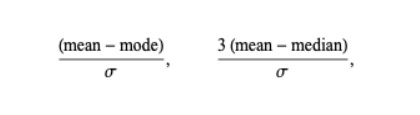
\includegraphics[width=9cm]{doc/latex/text/images/pearson-sk.jpg}
    \caption{Fórmulas para o 1º (esq.) e 2º (dir.) coeficientes de Pearson}
    \label{fig:pearson-sk}
\end{figure}


Quando uma distribuição é simétrica, ou seja, não possui valores em excesso tendendo acima ou abaixo da média, os coeficientes tendem a zero. Como exemplifica \citedirt{pearson1895}, há diversos fatores que podem influenciar na tendência de uma determinada variável:

\begin{citacao}
 Em primeiro lugar, o material medido pode ser heterogêneo e constituir de uma mistura de 2 ou mais materiais homogêneos. (...) A segunda classe de curvas de frequência ocorre no caso de material homogêneo quando a tendência de desvio para um lado de média é desigual a tendência para o outro lado. Curvas desse tipo aparecem em vários estudos físicos, econômicos e biológicos, por exemplo, em curvas de frequência para a altitude de um barômetro, em preços e taxas de juros de títulos mobiliários (...)
\end{citacao}

\section{Métodos de codificação}
Métodos comuns para representação codificada de dados categóricos no contento de \textit{Machine Learning} serão descritos nessa seção.

\subsection{One-hot encoding}
Método de codificação no qual cada valor é representado em sua forma codificada por um vetor de números inteiros no qual uma das posições corresponde ao valor 1 e todas as outras ao valor 0. \citedirt{google20} exemplifica o uso desse método com uma aplicação prática:

\begin{citacao}
Suponhamos que um dado \textit{dataset} de botânica descreva 15.000 diferentes espécies, cada uma indicada por uma \textit{string} identificadora única. Como parte da engenharia de parâmetros, você provavelmente codificaria esses identificadores como vetores \textit{one-hot}, os quais teriam tamanho 15.000.
\end{citacao}

\subsection{Embedding}
Método de codificação utilizado como alternativa ao \textit{one-hot encoding}. \citedirt{google20} define \textit{embedding} como "uma característica categórica representada como um valor contínuo" e "a tradução de um vetor de alta dimensionalidade para um espaço de baixa dimensionalidade". O mesmo autor exemplifica a aplicação prática do método:

\begin{citacao}
Você poderia representar as palavras em uma frase da língua Inglesa de duas maneiras: - Como um vetor esparso de milhões de elementos (alta dimensionalidade) no qual todos são valores inteiros. (...) - Como vários vetores densos de centenas de posições nos quais cada posição corresponde a um valor de ponto flutuante entre 0 e 1. Isso é um \textit{embedding}.
\end{citacao}

\section{Trabalhos Relacionados} \label{trabs-rel}
\label{trab-relacionados} 
No contexto de e-commerce, há trabalhos acadêmicos descrevendo diferentes abordagens, tais como sistemas de filtragem colaborativa que predizem avaliações por meio de fatorização de matrizes \cite{he17}, representam relações cliente/item utilizando grafos bipartidos \cite{wang19} e consideram fatores como críticas do usuário a sugestões geradas \cite{burke02} , sazonalidade e intenção de compra \cite{hwangbo18}.

Em sistema baseados em conteúdo ou com abordagens híbridas, é comum a utilização de resenhas escritas por usuários sobre os produtos como base para geração de sugestões, seja focando apenas na informação textual em si \cite{shoja19} ou relacionando com outros dados sobre os produtos em questão, tais como imagens \cite{wu20}.

Ainda no contexto de sistemas híbridos, há uma variedade de abordagens utilizadas para correlacionar produtos e clientes, tais como análise conjunta de múltiplos datasets e integração com dados provenientes de redes sociais \cite{li16}, cadeias de Markov \cite{yang20}, uso de agentes inteligentes baseados em lógica fuzzy \cite{yager00}, sistemas multi-agente \cite{aciar07}, entre outras.

No presente trabalho, em vez de trabalhar com avaliações numéricas dadas pelos usuários, as recomendações serão produzidas tendo com base somente no volume de vendas de um produto dentro de um determinado segmento de clientes. Isso permite que recomendações sejam geradas mesmo em aplicações que não coletam avaliações de clientes, ou em ERPs que possuem cadastros de pedidos simples, contando apenas com informações básicas do cliente, produto e transação, mas sem informações sobre a satisfação do consumidor no contexto pós-venda.

\textcolor{blue}{Padoin: vai citando mais trabalhos e no final precisamos dizer o que o teu tem de diferente dos demais}
\newline
\textcolor{blue}{Gabriel: alterei essa seção para citar mais trabalhos voltado a e-commerce e no último parágrafo destaco a diferença do meu para os demais}

\section{Considerações do Capítulo} \label{consid1}
Nesse capítulo foram apresentados áreas de conhecimento, tecnologias, técnicas e trabalho acadêmicos que possuem relação com o tema abordado nesse trabalho. No próximo capitulo serão apresentados os materiais e métodos e serem utilizados.

\chapter{Materiais e Métodos} \label{mat-metodos}
\pagestyle{simple} 

Nesse capítulo serão delimitados detalhes relativos à metodologia empregada para o desenvolvimento do trabalho, bem como especificidades do ambiente e ferramentas de \textit{software} a serem utilizadas.

\section{Metodologia Utilizada} \label{metodologia}

Visto que um dos objetivos do estudo é aplicar a IA treinada para gerar sugestões de produtos, esse se enquadra na classe de pesquisa qualitativa, ou seja, seus resultados irão nos ajudar a entender os comportamentos dos consumidores contidos na amostra de dados a ser utilizada. Contudo, a parametrização da rede neural muitas vezes envolve valores discretos, e como um dos objetivos é também encontrar a melhor configuração de rede para esse caso de uso, os resultados serão um misto de dados qualitativos e quantitativos.

Assim como descrito no trabalho de \citedir{burke02}, a proposta desse trabalho será desenvolver uma aplicação que gere sugestões com base em transações comerciais passadas, mas sem que haja a necessidade de que o comprador informe o tipo de produto que está buscando ou por qual motivo a compra ou pesquisa está sendo efetuada. A abordagem escolhida para atingir esse objetivo consiste no desenvolvimento de um sistema de recomendação híbrido. Como descrito na Seção \ref{sist-rec}, esse tipo de sistema integra características de diferentes abordagens, visando mitigar os problemas específicos de cada uma.

Inicialmente, será realizada a seleção da base de pedidos a ser utilizada para o treinamento da IA. Serão utilizados repositórios online como Kaggle, GitHub e UCI ML para buscar por conjuntos de dados. As bases escolhidas devem conter dados que permitam identificar clientes ou produtos de forma simples (ex.: nome, marca, categoria) e um código único para identificar essas entidades.

Após a seleção, serão definidos métodos que permitam inferir a popularidade de um produto em relação a um determinado cliente ou grupo de clientes. Essa popularidade será representado por uma avaliação numérica. Se uma combinação de cliente/produto recebe uma avaliação de valor alto, isso significará que o produto é uma boa recomendação para aquele cliente. Se a avaliação for baixa, isso significará que o produto pode não ser a recomendação mais adequada. Cada método definirá as avaliações de acordo com diferentes regras, agrupando os clientes por diferentes critérios.

Os \textit{datasets} selecionados no início do estudo serão processados por um algoritmo que aplicará as regras definidas pelos métodos, e para cada método o \textit{datases} de entrada resultará em outro de saída, contendo clientes, produtos e as avaliações inferidas. O conjunto de dados resultante desse projeto será utilizado para alimentar uma rede neural. As combinações de cliente/produto serão as entradas, e as avaliações serão as saídas. 

A rede neural será criada através da biblioteca Keras em Python. Utilizando o editor Jupyter Notebook será possível prototipar uma estrutura inicial e testá-la até chegar em um código minimamente funcional, uma rede que possa ser treinada e que retorne predições corretas, ainda que considerando apenas uma fração do conjunto de dados total. 

Desse ponto em diante, o desenvolvimento será realizado utilizando o Visual Studio Code. Diferente do Jupyter, que organiza o código em "células" e permite a inclusão de comentários com texto formatado, imagens e outros recursos visuais junto ao código, o Visual Studio Code funciona de forma mais parecida com um editor de texto convencional. Esse ambiente permite que o código seja organizado com mais concisão e clareza, o que se torna importante à medida que o projeto avança e o número de linhas cresce.

Se necessário, a rede neural passará então por diversas iterações de treinamento, na qual serão testados diferentes parametrizações referentes ao processo de treinamento em si (ex.: número de épocas, \textit{batch size}) ou à rede (ex.: número de neurônios, camadas e funções de ativação, erro e otimização). Cada teste será registrado de modo que possam ser identificadas as configurações que resultem nos modelos mais precisos e rápidos. Ao final dos testes, os melhores modelos serão utilizados para a geração de sugestões.

Por fim, as avaliações e sugestões geradas por cada método serão comparadas e então analisadas qualitativamente em relação aos dados que as originaram. Ou seja, a partir de uma análise manual dos dados, será possível constatar se as previsões geradas foram relevantes ou não. Caso não sejam, novos testes serão realizados até que seja encontrado o modelo ideal. Essa pesquisa possui, portanto, caráter aplicado e exploratório.

\section{Ambiente de Testes} \label{amb-testes}
Para desenvolvimento e prototipação foi utilizado um notebook Acer Nitro 5 com as seguintes configurações de \textit{hardware}:
\begin{itemize}
    \item Processador: Intel Core i5-8300H @ 2.30GHz, 4 núcleos, 8 processadores lógicos
    \item RAM: 8GB
    \item Armazenamento: 1TB
\end{itemize}

O seguinte ambiente de \textit{software} foi configurado no notebook:
\begin{itemize}
    \item Sistema Operacional: Windows 10 Education
    \item Versão do Python: 3.7.6
    \item Editor de texto: Jupyter Notebook v6.0.3
\end{itemize}

Os testes descritos no trabalho foram efetuados em um servidor da Unijuí com  com as seguintes configurações de \textit{hardware}:
\begin{itemize}
    \item Processador: Intel Core i7-8700 @ 3.20GHz, 6 núcleos, 12 processadores lógicos
    \item RAM: 16GB
    \item Armazenamento: 450GB
\end{itemize}

O seguinte ambiente de \textit{software} foi configurado no servidor:
\begin{itemize}
    \item Sistema Operacional: Ubuntu 18.04.4 LTS
    \item Versão do Python: 3.6.9
    \item Editor de texto: nano
\end{itemize}

\section{Considerações do Capítulo} \label{consid2}
Nesse capítulo foram apresentadas as metodologias empregadas no desenvolvimento do trabalho, bem como especificidades do ambiente de desenvolvimento e ferramentas, tanto no âmbito do \textit{software} quanto do \textit{hardware}. 

\chapter{Desenvolvimento} \label{desenv}
\pagestyle{simple} 

Nessa seção serão descritas de forma mais detalhada as etapas de análise dos datasets e os processos realizados em cada etapa, visando descrever como as recomendações foram obtidas através do uso das ferramentas e técnicas descritas nas seções anteriores.

\section{Escolha do dataset} \label{escolha-ds}

Para o trabalho foram escolhidos 3 \textit{datasets} de \textit{e-commerce} entre dezenas disponíveis nos repositórios Kaggle e UCI ML. Estes conjuntos foram escolhidos pois possuem características que favorecem sua utilização para testes de sistemas de recomendação, tais como:

\begin{itemize}
    \item Estão disponíveis de forma integral, pública e gratuita
    \item Possuem mais de 100 mil registros
    \item Embora os clientes estejam anonimizados, os conjuntos mantém dados que permitem categorizá-los (ex.: cidade/estado/país de origem)
    \item Os datasets provenientes do UCI ML já foram utilizados com propósitos acadêmicos por \citedir{chen10}
    \item O dataset proveniente do Kaggle recebeu boas avaliações: possui classificação "Ouro" pela plataforma, ganhou 1023 votos positivos de usuários e "Usabilidade" avaliada como nota 10/10. \footnote{Dados referentes ao dia 19/09/2020}
\end{itemize}

\begin{table}[ht]
\centering
\begin{tabular}{@{}lllll@{}}
\toprule
\textbf{Nome}        & \textbf{Nº de registros} & \textbf{Tamanho (MB)} & \textbf{Período} & \textbf{Origem} \\ \midrule
Online Retail        & 541.909                  & 43,4                  & 2010-2011        & UCI ML             \\
Online Retail II     & 1.067.371                & 85,7                  & 2009-2011        & UCI ML            \\
Brazilian E-Commerce & 112.650                   & 7,5                  & 2016-2018        & Kaggle          \\ \bottomrule
\end{tabular}
\caption{Dados sobre os datasets selecionados para o trabalho}
\label{tab:my-table}
\end{table}

\section{Estudo de sistemas de recomendação} \label{estudo-sist}
Decidiu-se por seguir um modelo de filtragem colaborativa, que tal como descrito na Seção \ref{sist-rec} leva em conta apenas as avaliações dadas pelos clientes a um determinado produto e não dados do produto em si. Contudo, há diferentes maneiras de implementar sistemas de desse tipo e portanto antes de iniciar-se o desenvolvimento foi realizada uma busca por tutoriais e projetos de exemplo na Internet que explicassem mais detalhadamente essas implementações. 

Em um dos projetos encontrados, \citedir{tanner18} explica em vídeo uma abordagem semelhante na qual ele treina e testa um modelo de sugestão de livros baseado em avaliações (notas de 1 a 5) das pessoas que os compraram. A rede criada por ele é treinada de forma a aprender a relação entre essas entradas categóricas e suas respectivas saídas, as avaliações, como exemplificado na figura \ref{fig:tanner}.

Nesse trabalho, optou-se por seguir a implementação de Tanner, visto que esta apresenta várias vantagens do ponto de vista de desempenho e manutenção de código que serão explicadas em mais detalhes na Seção \ref{geracao-rec}.

\begin{figure}[htp]
    \centering
    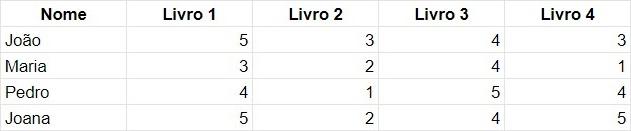
\includegraphics[width=12cm]{doc/latex/text/images/tanner.jpg}
    \caption{Exemplo do sistema de recomendação de Tanner}
    \label{fig:tanner}
\end{figure}

\section{Definição de critério de avaliação} \label{definicao-crit}
Para que se possa utilizar a abordagem ilustrada por \citedir{tanner18} com qualquer \textit{datasets}, é necessário que avaliações numéricas (por exemplo, notas de 1 a 5) estejam relacionadas às transações analisadas. Contudo, não é todo \textit{dataset} que possui esse tipo de dado. Os conjuntos listados na Seção \ref{escolha-ds}, por exemplo, elencam somente pares de clientes/produtos, e portanto o único dado que pode ser inferido desses \textit{datasets} é a frequência de compra por cliente. Visto que não há informação detalhada sobre o produto, abordagens baseadas em conteúdo (características do produto) ou objetivos (para quê o produto serve) não são viáveis.

Foram portanto definidos 3 métodos de criar avaliações para os registros nesses \textit{datasets}, baseados na frequência de compra em diferentes agrupamentos de clientes. Quanto mais popular um produto é, mais passível de recomendação ele se torna. As regras de avaliação foram baseadas nas definições para filtragem colaborativa (FC) no contexto de sistemas de recomendação. 

\begin{itemize}
   \item FC por Categoria: se o cliente não comprou e o produto é popular dentro da categoria na qual o cliente está, define avaliação alta. Isso aumenta a probabilidade de recomendação para produtos populares na categoria (Figura \ref{fig:fc-categ}).
    \item FC Intercategorias: se o cliente em questão não comprou o produto e este é popular dentro da categoria do cliente, define avaliação alta. Se o cliente não comprou, o produto não é popular, mas outro cliente da mesma categoria comprou, define avaliação média. Isso aumenta a probabilidade de recomendação para produtos populares na categoria enquanto também destaca produtos menos populares adquiridos por clientes similares. (Figura \ref{fig:fc-intercateg}).
    \item FC Geral: segue as mesmas regras do FC por Categoria, mas considerando a popularidade dos produtos entre todos os clientes. Nesse caso, se o cliente não comprou o produto e este é popular no geral, define avaliação alta. Isso aumenta a probabilidade de recomendação para produtos populares no geral.
\end{itemize}

\begin{figure}[htp]
    \centering
    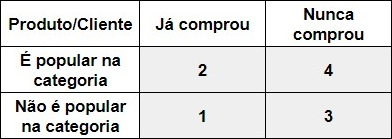
\includegraphics[width=12cm]{doc/latex/text/images/fc-categ.jpg}
    \caption{Avaliação FC geral ou por categoria.}
    \label{fig:fc-categ}
\end{figure}

\begin{figure}[htp]
    \centering
    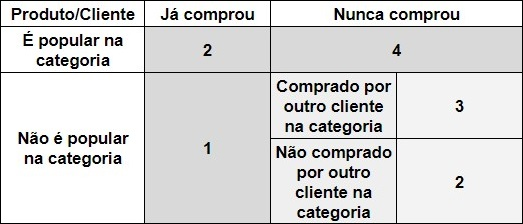
\includegraphics[width=12cm]{doc/latex/text/images/fc-intercateg.jpg}
    \caption{Avaliação FC por intercategorias}
    \label{fig:fc-intercateg}
\end{figure}

Tendo os métodos de avaliação definidos, sua lógica foi descrita em \textit{scripts} Python. Cada \textit{script} contém instruções para percorrer todos os registros em cada um dos \textit{datasets} selecionados, analisar os produtos mais vendidos de acordo com uma categorização de cliente e produzirem um \textit{dataset} de saída contendo 3 colunas: código do cliente, código do produto e avaliação.

No caso dos \textit{datasets} provenientes do repositório UCI ML, decidiu-se categorizar os clientes com base na coluna \textit{country} (país de origem). No caso do conjunto do Kaggle, que aborda transações exclusivamente realizadas no Brasil, a coluna \textit{customer\_state} (UF de origem) serviu de base para categorização de clientes.

Após terem sido produzidas avaliações para os 3 \textit{datasets} selecionados, esses valores foram analisados sob o ponto de vista da estatística descritiva, de forma a entender como cada método avaliou os dados contidos no dataset. O resultados dessa análise serão explicados em mais detalhes na Seção \ref{resultados}.

\section{Geração de recomendações} \label{geracao-rec}
Após a geração de avaliações conforme os métodos definidos na Seção \ref{definicao-crit}, os \textit{datasets} resultantes foram utilizados como entrada para o treinamento da rede neural descrita por Tanner. A rede consiste em 4 camadas iniciais, que fazem o processo de \textit{embedding} dos produtos e clientes, e 3 camadas do tipo Dense, que permitem à rede relacionar as entradas categóricas com as avaliações durante o treinamento.

\begin{figure}[htp]
    \centering
    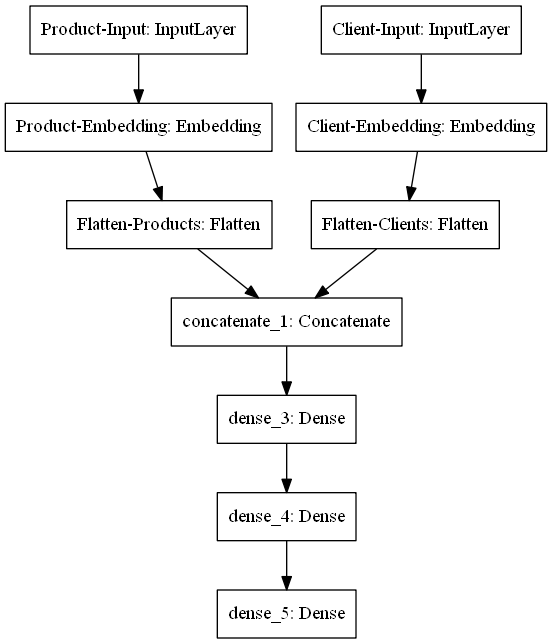
\includegraphics[width=10cm]{doc/latex/text/images/network.png}
    \caption{Estrutura de rede neural utilizada}
    \label{fig:fc-intercateg}
\end{figure}

Essa estrutura de rede foi escolhida para o trabalho pois apresenta as seguintes vantagens:

\begin{itemize}
    \item Conforme detalhado na Seção \ref{sist-rec}, o uso de \textit{embeddings} em \textit{Machine Learning} permite a redução de dimensionalidade e por consequência uma melhor utilização de recursos computacionais tais como memória RAM e processamento
    \item Consolida o processo de criação e aprendizado do \textit{embedding} na mesma estrutura, facilitando o entendimento e manutenção do código.
    \item O funcionamento da estrutura foi documentado pelo autor tanto em texto quanto em vídeo, o que permite entendê-lo e comprová-lo de forma mais assertiva.
\end{itemize}

A rede neural foi treinada utilizando um \textit{dataset} de entrada de cada vez. Após o treinamento, a rede foi testada manualmente com pares de produtos/clientes do \textit{dataset} para atestar que o treinamento ocorreu de forma bem sucedida.
\chapter{Resultados} \label{resultados}

\section{Avaliações}
Após terem sido geradas para todos os datasets, as medidas estatísticas de posição e dispersão dessa avaliações foram compiladas (Tabela \ref{tab:analise-ds}). A partir da análise do 1º coeficiente de Pearson, pode-se concluir que as avaliações para todos os conjuntos apresentaram assimetria negativa, ou seja, valores de avaliação altos aparecem com mais frequência na amostra do que os baixos. Isso se comprova na observação da mediana e moda, que foi maior ou igual a 3 para todos os datasets.

A partir desses dados, pode-se concluir que os produtos presentes nos datasets analisados apresentaram alto volume de vendas na maioria dos casos. Caso houvesse um dataset repleto de produtos com baixo volume de vendas, as avaliações teriam comportamento inverso, tendendo a valores mais baixos (assimetria positiva).

\begin{table}[ht]
\begin{tabular}{@{}llrrrr@{}}
\toprule
\multicolumn{1}{c}{\textbf{Método}} & \multicolumn{1}{c}{\textbf{Dataset}} & \multicolumn{1}{c}{\textbf{Média}} & \multicolumn{1}{c}{\textbf{Mediana}} & \multicolumn{1}{c}{\textbf{Moda}} & \multicolumn{1}{l}{\textbf{Coef. Pearson}} \\ \midrule
FC-Inter-Categoria                  & Brazilian retail                     & 3,41377                            & 4                                    & 4                                 & -184,38\%                                  \\
FC-Geral                            & Brazilian retail                     & 3,52950                            & 4                                    & 4                                 & -174,78\%                                  \\
FC-Categoria                        & Brazilian retail                     & 3,55913                            & 4                                    & 4                                 & -167,57\%                                  \\
FC-Inter-Categoria                  & Online Retail 1                      & 2,89565                            & 3                                    & 3                                 & -87,41\%                                   \\
FC-Inter-Categoria                  & Online Retail 2                      & 2,90716                            & 3                                    & 3                                 & -84,47\%                                   \\
FC-Geral                            & Online Retail 1                      & 2,99107                            & 3                                    & 3                                 & -13,03\%                                   \\
FC-Categoria                        & Online Retail 1                      & 2,99187                            & 3                                    & 3                                 & -11,77\%                                   \\
FC-Geral                            & Online Retail 2                      & 2,99361                            & 3                                    & 3                                 & -11,06\%                                   \\
FC-Categoria                        & Online Retail 2                      & 2,99415                            & 3                                    & 3                                 & -10,02\%                                   \\ \bottomrule
\end{tabular}
\caption{Atributos estatísticos das previsões geradas}
\label{tab:analise-ds}
\end{table}

Também para determinar se as avaliações pertencem a uma distribuição normal, a amostra foi analisada utilizando o teste de Anderson-Darling. O valor obtido foi de 1811063,02. Para um intervalo de confiança de 95\%, pode-se rejeitar a hipótese de normalidade dos dados. 

\textcolor{blue}{Gabriel: o teste que fiz com o coeficiente de pearson não é suficiente para determinar que a distribuição não é normal? é preciso definir esses testes na fundamentação?}

\section{Recomendações - Cenário 1} \label{cenario1}
No primeiro cenário de testes, recomendações foram geradas para o \textit{dataset} Online Retail utilizando a abordagem de FC por categoria. Nesse caso, o critério considerado para a categorização foi o país de origem do cliente.

Os 5 produtos que mais receberam avaliação 4 conforme a análise constam na Tabela \ref{tab:a4}. Nessa amostra, todos os produtos foram considerados boas recomendações para 8 em cada 10 clientes da base. A partir disso, pode-se concluir que esse produtos possuem alta demanda em todos os países analisados. Os produtos nessa amostra, assim como os demais no \textit{dataset}, são itens de utilidade doméstica (bandeja e potes para bolo e sacolas térmicas para alimentos).

Quanto aos produtos que mais frequentemente receberam avaliação 3 (Tabela \ref{tab:a3}), pode-se concluir que foram os mesmos para todos os clientes. Isso indica que há produtos no conjunto que não foram adquiridos por nenhum cliente, e que por consequência também não figuraram entre os mais vendidos nos países de origem dos clientes. Esses produtos correspondem a 27,22\% do total, ou seja, essa amostra engloba 1108 dos 4070 produtos presentes na base.

Analisando os produtos que mais frequentemente receberam avaliações 2 e 1 (Tabelas \ref{tab:a2} e \ref{tab:a1}), pode-se concluir que o produto que mais frequentemente recebeu notas baixas foi assim avaliado para somente 4,6\% dos clientes. Esse cenário indica que a maior parte dos produtos na base é vendido com frequência igual ou próxima, enquanto somente uma parcela menor tem baixo de volume venda em cada país analisado. Essa análise, portanto, condiz também com a encontrada para os itens com avaliação 3.

Portanto, pode-se concluir que a abordagem de FC por Categoria aplicada ao \textit{dataset} citado trabalhou de forma a avaliar com pontuação alta todos os produtos populares nos países analisados, e com valor ligeiramente mais baixo os produtos que nenhum dos clientes comprou. Dessa forma, o sistema de recomendação é capaz de incentivar clientes antigos a recomprarem produtos populares, clientes novos a comprarem esses mesmos produtos, bem tornar produtos com baixo volume de venda mais populares entre a base de consumidores como um todo. Todos esses cenários são positivos para os vendedores que ofertam seus itens em \textit{e-commerce}.

\vspace{1cm}

\begin{table}[ht]
\centering
\begin{tabular}{@{}llll@{}}
\toprule
\textbf{ID produto} & \textbf{Nome produto}         & \textbf{Nº avaliações 4} & \textbf{\% clientes} \\ \midrule
180                 & LUNCH BAG RED RETROSPOT          & 3916                          & 89,55                       \\
1348                & REGENCY CAKESTAND 3 TIER         & 3866                          & 88,41                       \\
1314                & LUNCH BAG SUKI DESIGN            & 3827                          & 87,51                       \\
182                 & LUNCH BAG BLACK SKULL            & 3818                          & 87,31                       \\
1631                & SET OF 3 CAKE TINS PANTRY DESIGN & 3806                          & 87,03                       \\ \bottomrule
\end{tabular}
\caption{Análise dos 5 produtos que mais receberam avaliação 4}
\label{tab:a4}
\end{table}
\vspace{1cm}

\begin{table}[ht]
\centering
\begin{tabular}{@{}llll@{}}
\toprule
\textbf{ID produto} & \textbf{Nome produto}         & \textbf{Nº avaliações 3} & \textbf{\% clientes} \\ \midrule
4068       & GIFT VOUCHER £50.00  & 4373                 & 100,00             \\
2610       & BIG POLKADOT MUG                    & 4373                 & 100,00             \\
2601       & CHRISTMAS TREE T-LIGHT HOLD & 4373                 & 100,00             \\
2600       & FOLKART HEART NAPKIN RINGS          & 4373                 & 100,00             \\
2603       & ART METAL HEART T-LIGHT HOLDER & 4373                 & 100,00             \\ \bottomrule
\end{tabular}
\caption{Análise dos 5 produtos que mais receberam avaliação 3}
\label{tab:a3}
\end{table}
\vspace{1cm}

\begin{table}[ht]
\centering
\begin{tabular}{@{}llll@{}}
\toprule
\textbf{ID produto} & \textbf{Nome produto}         & \textbf{Nº avaliações 2} & \textbf{\% clientes} \\ \midrule
3536       & HANGING HEART T-LIGHT HOLDER & 432                  & 9,88               \\
1348       & REGENCY CAKESTAND 3 TIER           & 393                  & 8,99               \\
3305       & ASSORTED COLOUR BIRD ORNAMENT      & 339                  & 7,75               \\
4062       & POSTAGE                            & 253                  & 5,79               \\
3515       & JUMBO BAG RED RETROSPOT            & 229                  & 5,24               \\ \bottomrule
\end{tabular}
\caption{Análise dos 5 produtos que mais receberam avaliação 2}
\label{tab:a2}
\end{table}
\vspace{1cm}

\begin{table}[ht]
\centering
\begin{tabular}{@{}llll@{}}
\toprule
\textbf{ID produto} & \textbf{Nome produto}         & \textbf{Nº avaliações 1} & \textbf{\% clientes} \\ \midrule
339        & REX CASH+CARRY JUMBO SHOPPER    & 208                  & 4,76               \\
1862       & JAM MAKING SET WITH JARS        & 179                  & 4,09               \\
1043       & PAPER CHAIN KIT 50'S CHRISTMAS  & 172                  & 3,93               \\
1128       & VICTORIAN GLASS HANGING T-LIGHT & 170                  & 3,89               \\
3346       & ANTIQUE SILVER TEA GLASS ETCHED & 160                  & 3,66               \\ \bottomrule
\end{tabular}
\caption{Análise dos 5 produtos que mais receberam avaliação 1}
\label{tab:a1}
\end{table}
\vspace{1cm}
\chapter{Conclusão}
\label{conclusão}

Neste capítulo serão apresentadas as conclusões obtidas no desenvolvimento do presente trabalho, bem como possibilidades de expansão do estudo em trabalhos futuros.

\section{Conclusão}
Este trabalho apresentou o desenvolvimento de um sistema de recomendação de produtos para \textit{e-commerce} com utilização de técnicas de IA e ML aliadas com análise estatística. O sistema descrito sugere produtos com base em diferentes análises da relação entre o volume de vendas de um item e os clientes e segmentos relacionados a essa venda. Em trabalhos futuros, pretende-se validar esse modelo através de sua implementação em uma aplicação de \textit{e-commerce} real, bem como testar diferentes abordagens para geração de avaliações e recomendações.



% ----------------------------------------------------------
% ELEMENTOS PÓS-TEXTUAIS
% ----------------------------------------------------------
\postextual

% ----------------------------------------------------------
% Referências bibliográficas
% ----------------------------------------------------------
\bibliography{abntex2-modelo-references}

% ----------------------------------------------------------
% Anexos
% ----------------------------------------------------------
\begin{anexosenv}
\partanexos

\chapter{Código - Rede neural Dense do Keras} \label{anexo1}
\begin{lstlisting}
    import pandas as pd
    from keras.models import Model
    from keras.layers import Input, Embedding, Flatten, Dense, Concatenate
    from sklearn.model_selection import train_test_split
 
    # carregar arquivo, dividir dataset em treinamento/teste
    dataset = pd.read_csv('arquivo.csv')
    train, test = train_test_split(dataset, test_size=0.2, random_state=42)

    # criar embedding para produtos
    prod_input = Input(shape=[1], name="Prod-Input")
    prod_embedding = Embedding(n_prods+1, 5, name="Prod-Embedding")(prod_input)
    prod_vec = Flatten(name="Flatten-Prods")(prod_embedding)
    
    # criar embedding para segmentos de cliente
    client_input = Input(shape=[1], name="Client-Input")
    client_embedding = Embedding(n_users+1, 5, name="Client-Embedding")(client_input)
    client_vec = Flatten(name="Flatten-Clients")(client_embedding)
    
    # concatenar conjuntos
    conc = Concatenate()([prod_vec, client_vec])
    
    # adicionar camadas
    fc1 = Dense(128, activation='relu')(conc)
    fc2 = Dense(32, activation='relu')(fc1)
    out = Dense(1)(fc2)
    
    # treinamento
    model2 = Model([client_input, prod_input], out)
    model2.compile('adam', 'mean_squared_error')
\end{lstlisting}

\end{anexosenv}

%-------------------------------------------------------------------
% INDICE REMISSIVO
%-------------------------------------------------------------------
\phantompart
\printindex

\end{document}
